\documentclass[12pt]{article}
\usepackage{geometry}                % See geometry.pdf to learn the layout options. There are lots.
\geometry{letterpaper}                   % ... or a4paper or a5paper or ... 
%\geometry{landscape}                % Activate for for rotated page geometry
\usepackage[parfill]{parskip}    % Activate to begin paragraphs with an empty line rather than an indent
\usepackage{daves,fancyhdr,natbib,graphicx,dcolumn,amsmath,lastpage,url}
\usepackage{amsmath,amssymb,epstopdf,longtable}
\usepackage[final]{pdfpages}
\DeclareGraphicsRule{.tif}{png}{.png}{`convert #1 `dirname #1`/`basename #1 .tif`.png}
\pagestyle{fancy}
\lhead{CE 3354 -- Engineering Hydrology}
\rhead{FALL 2024}
\lfoot{ES6}
\cfoot{}
\rfoot{Page \thepage\ of \pageref{LastPage}}
\renewcommand\headrulewidth{0pt}
% other
\usepackage{paralist}  % need to modify standard enumerate blocks
%=========Longtable environment
\usepackage{setspace}                % allow single and double space environment
\usepackage{longtable}                % allow table to span multiple pages
\usepackage{caption}                    % consistent caption package
\usepackage{url}					% Ubiquitious url formatting package
%===========

\DeclareGraphicsRule{.tif}{png}{.png}{`convert #1 `dirname #1`/`basename #1 .tif`.png}
%++++++++++++++++++++++++++++++++++++++++++++++++++++++++++++++++++++++++++


\begin{document}
\begin{center}
{\textbf{{ CE 3354 Engineering Hydrology} \\ {Exercise Set 6}}}
\end{center}

 \section*{\small{Exercises}}
 \begin{enumerate}
%\item Problem 7.3.5 in Mays, pg. 278.

\item An agricultural watershed was urbanized over a 20 year interval.  A triangular one-hour unit hydrograph was developed for this watershed for an excess rainfall duration of one hour.  

Before urbanization, the average loss rate was 0.30 in/hr.  

Figure \ref{fig:UnitGraph1} is the unit hydrograph that has a peak discharge of 400 cfs/in occurring at 3 hours, and a base time of 9 hours.
\begin{figure}[h!] %  figure placement: here, top, bottom, or page
   \centering
   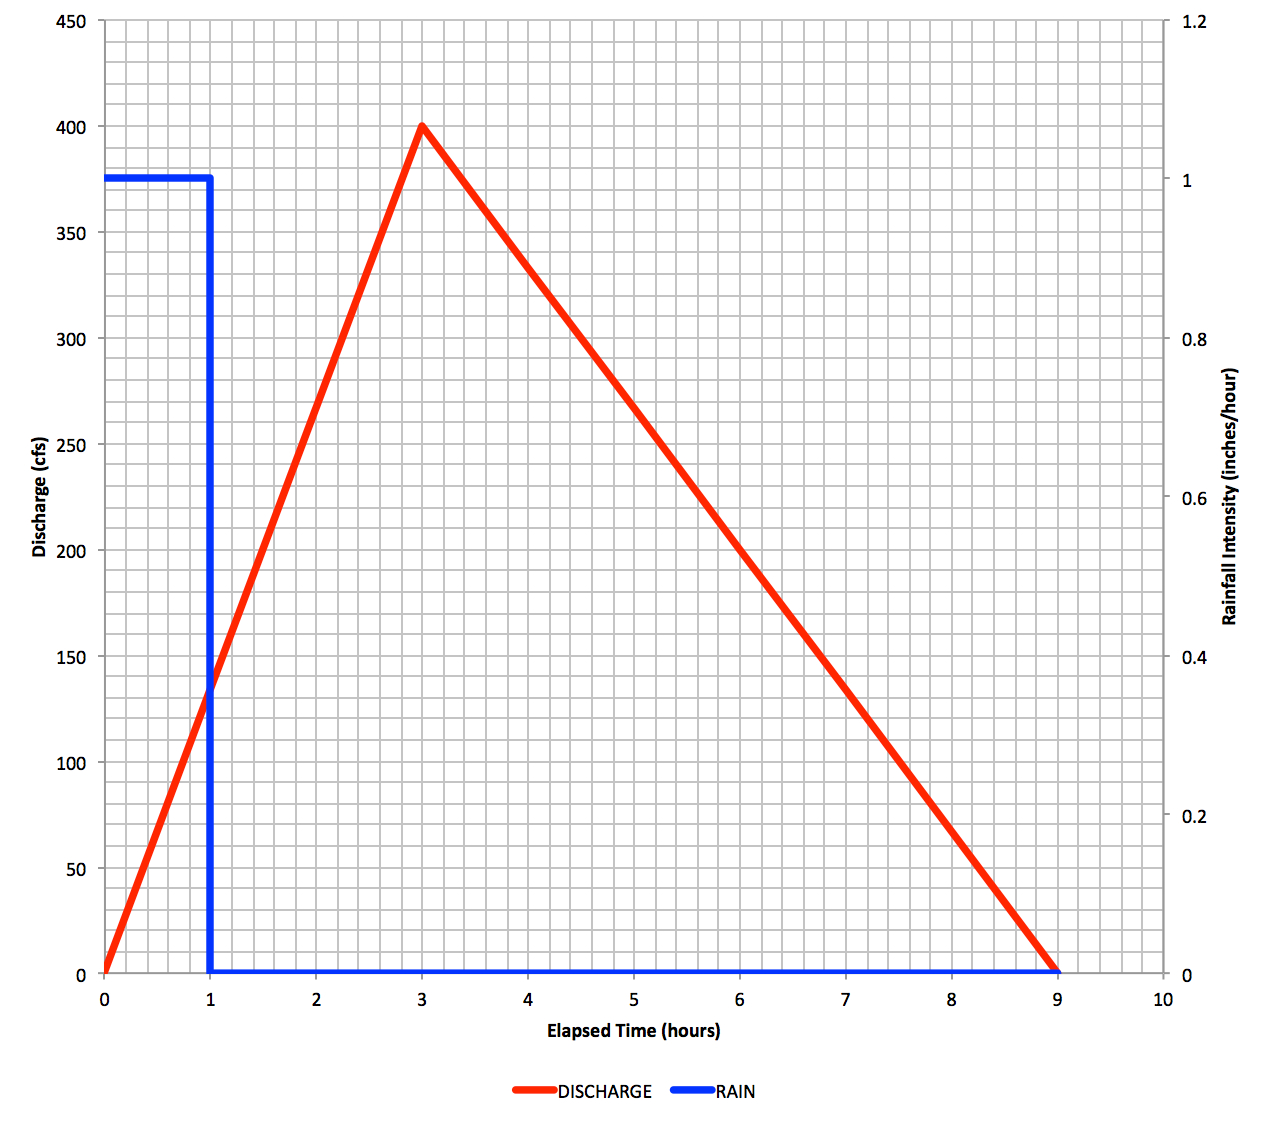
\includegraphics[width=5in]{UnitGraph1.jpg} 
   \caption{Pre-Urbanization unit hydrograph for excess rainfall of 1 in/hr for 1 hour.}
   \label{fig:UnitGraph1}
\end{figure}
\clearpage

After urbanization the loss rate was reduced to 0.15 in/hr and the peak discharge of the unit hydrograph increased to 600 cfs/in occurring at 1 hour, and the base time reduced to 6 hours.    Figure \ref{fig:UnitGraph2} is the unit hydrograph with a peak discharge of 600 cfs occurring at 1 hours, and a time base of 6 hours.

\begin{figure}[h!] %  figure placement: here, top, bottom, or page
   \centering
   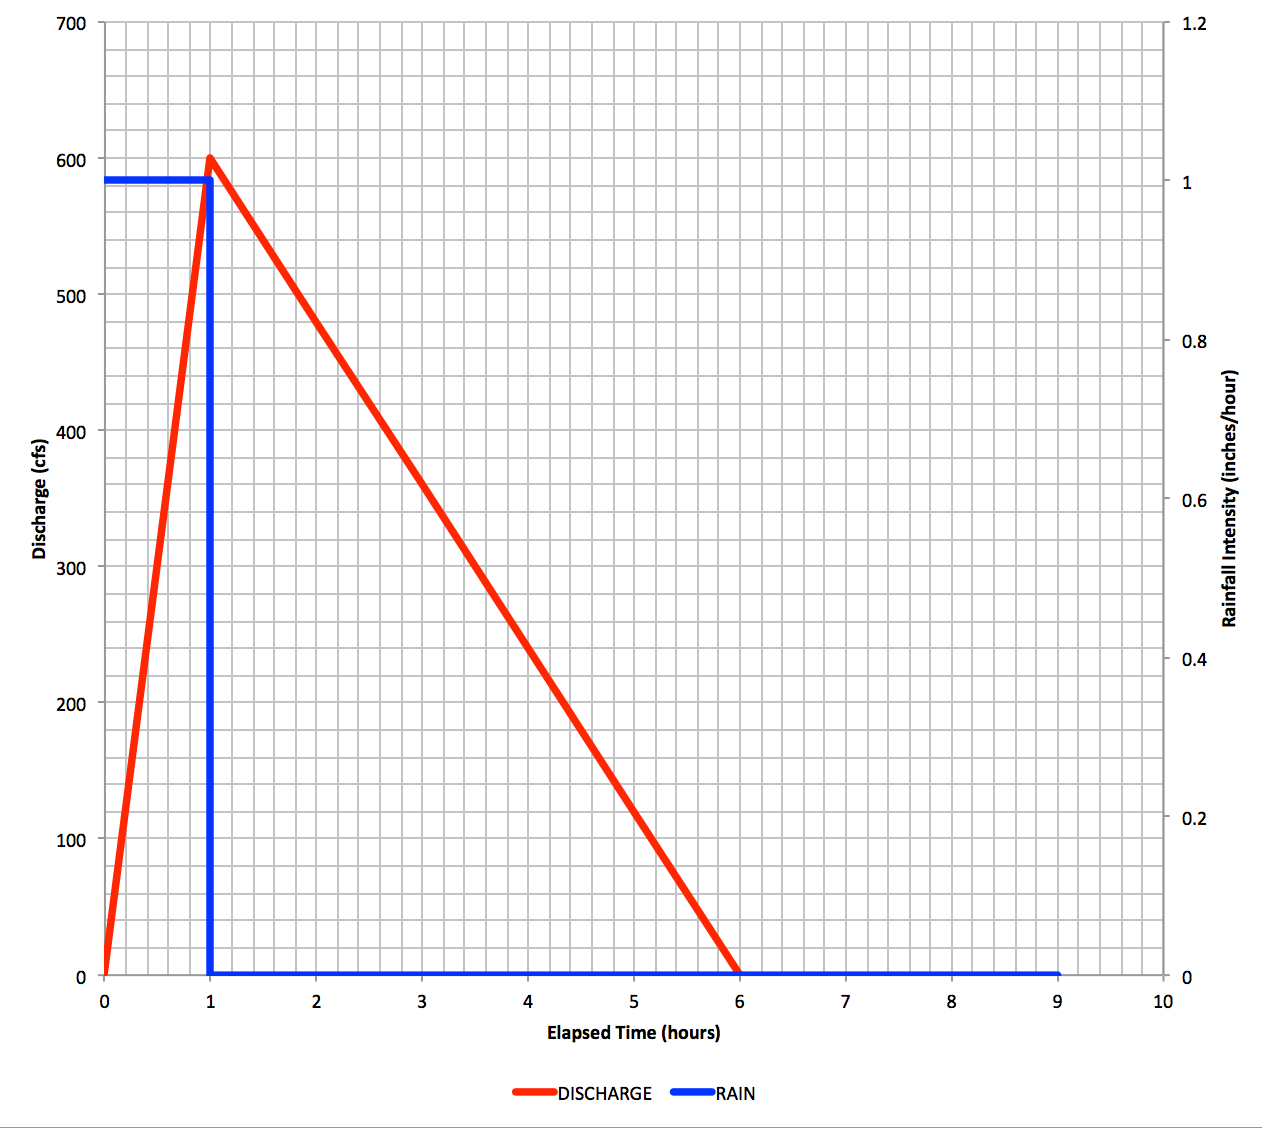
\includegraphics[width=5in]{UnitGraph2.jpg} 
   \caption{Post-Urbanization unit hydrograph for excess rainfall of 1 in/hr for 1 hour.}
   \label{fig:UnitGraph2}
\end{figure}

For a two hour storm in which 1 inch of rain fell in the first hour and 0.5 inch in the second hour, determine the direct runoff hydrographs before and after urbanization.\footnote{This exercise is the same as problem 7.5.7, pg. 238 in Chow, Maidment, Mays}

\clearpage
%%%%%%%%%%%%%%%%%%%%%%%%%%%%%%%%
\textbf{Solution}

\begin{enumerate}[a)]

\item Using Figure \ref{fig:UnitGraph1} as a template, the two increments of rainfall are directly plotted onto the template, then loss is applied to each increment.  The resulting unitgraphs from each increment are plotted (in magenta/purple) and then ordinate-by-ordinate addition is used to construct the composite direct runoff hydrograph, as depicted in Figure \ref{fig:PreUrban}

\begin{figure}[h!] %  figure placement: here, top, bottom, or page
   \centering
   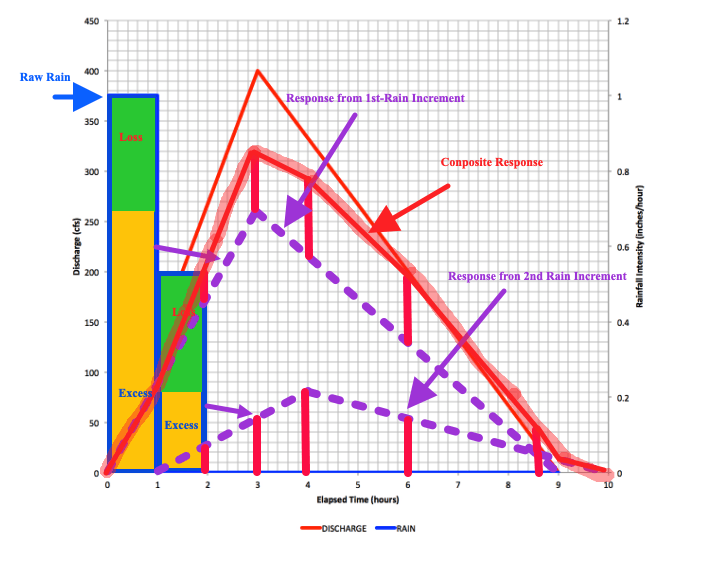
\includegraphics[width=6in]{PreUrban.png} 
   \caption{Pre-Urbanization unit hydrograph for excess rainfall of 1 in/hr for 1 hour.}
   \label{fig:PreUrban}
\end{figure}

\clearpage
%%%%%%%%%%%%%%%%%%%%%%%%%%%%%%%%%

\item Using Figure \ref{fig:UnitGraph2} as a template, the two increments of rainfall are directly plotted onto the template, then loss is applied to each increment.  The resulting unitgraphs from each increment are plotted (in magenta/purple) and thenordinate-by-ordinate addition is used to construct the composite direct runoff hydrograph, as depicted in Figure \ref{fig:PostUrban}

\begin{figure}[h!] %  figure placement: here, top, bottom, or page
   \centering
   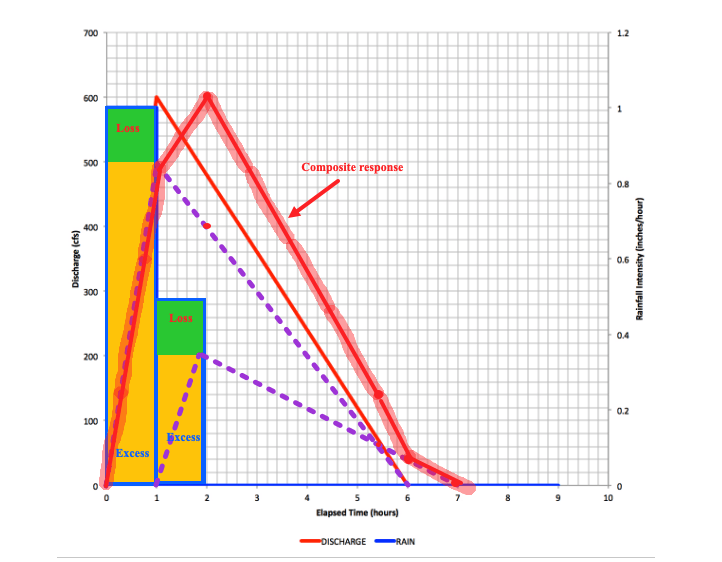
\includegraphics[width=6in]{PostUrban.png} 
   \caption{Post-Urbanization unit hydrograph for excess rainfall of 1 in/hr for 1 hour.}
   \label{fig:PostUrban}
\end{figure}

\clearpage
%%%%%%%%%%%%%%%%%%%%%%%%%%%%%%%%%%%

\item Alternatively (and more usefully) the responses can be incorporated into a spreadsheet as depicted in Figure \ref{fig:UHfromDrawings}.

\begin{figure}[h!] %  figure placement: here, top, bottom, or page
   \centering
   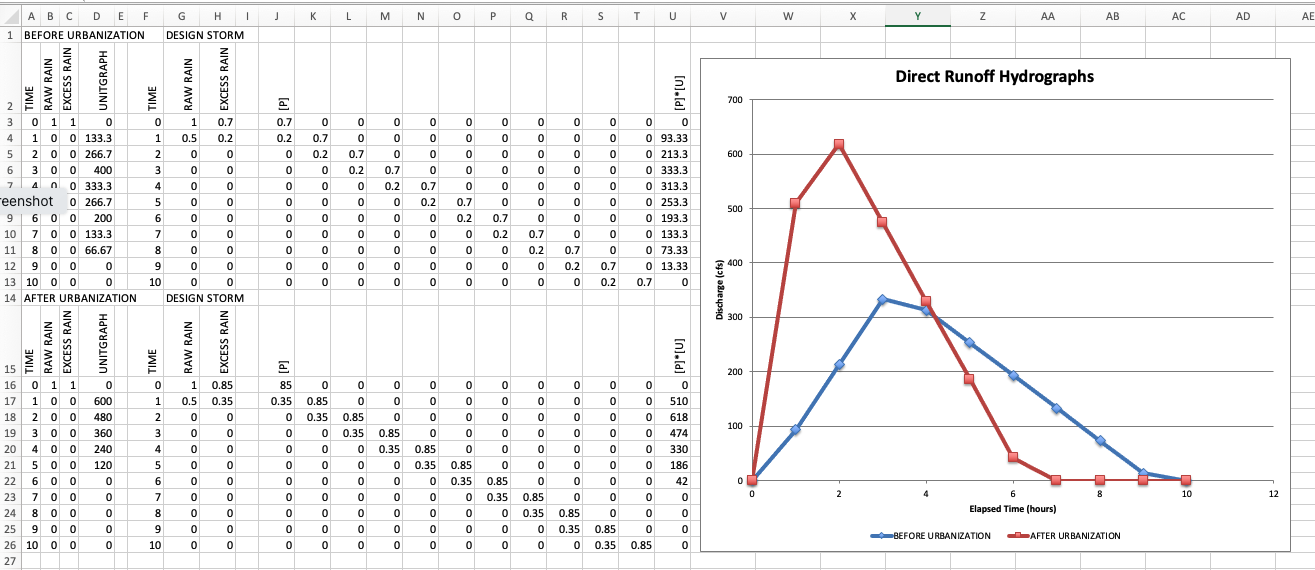
\includegraphics[width=6in]{UHfromDrawings.png} 
   \caption{Spreadsheet solution}
   \label{fig:UHfromDrawings}
\end{figure}

The working spreadsheet is located at \url{http://54.243.252.9/ce-3354-webroot/2-Exercises/ES-6/ES6-SourceCode/ES6-Solution.xlsx}. Figure \ref{fig:UHfromDrawings} is captures from Tab Sheet ``P1.''

\end{enumerate}
\clearpage
%%%%%%%%%%%%%%%%%%%%%%%%%%%%%%%%%%

\item A storm on April 16, 1977, on the Shoal Creek watershed at Northwest Park in
Austin, Texas, resulted in the rainfall-runoff values in Figure \ref{fig:RainRunoff1}.

Use the linear regression method to determine the half-hour unit hydrograph for the watershed. 
The watershed drainage area is 7.03 $mi^2$.
Assume that a uniform loss rate (constant loss model) is valid.\footnote{This exercise is a hybrid of problems 7.6.2 and 7.6.5, pg  239 in Chow, Maidment, and Mays.}

\begin{figure}[h!] %  figure placement: here, top, bottom, or page
   \centering
   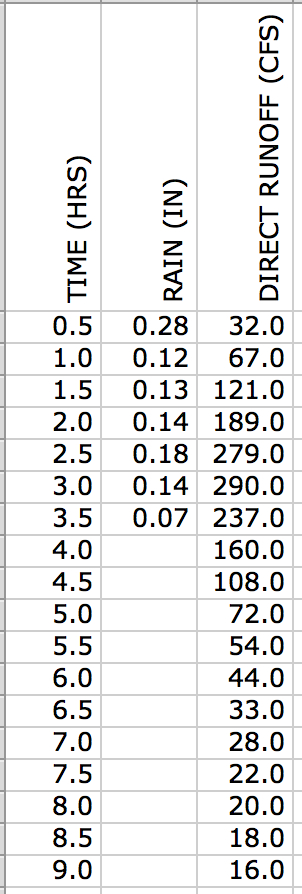
\includegraphics[width=1.5in]{RainRunoff1.jpg} 
   \caption{Observed storm rainfall incremental depths and observed direct runoff hydrograph}
   \label{fig:RainRunoff1}
\end{figure}

\clearpage
%%%%%%%%%%%%%%%%%%%%%%%%%%%%%%%%
\textbf{Solution}

\begin{enumerate}[a)]

\item Using data from Figure \ref{fig:RainRunoff1} and the supplied watershed area, the rainfall is converted into watershed input volume in same units as watershed runoff volume.  A constant loss is applied to the rainfall increments until the ratio of output to input is unity.  as a template, the two increments of rainfall are directly plotted onto the template, then loss is applied to each increment.  Predict-and-correct or Goal Seek is sufficient as depicted in Figure \ref{fig:VolumeBalance}

\begin{figure}[h!] %  figure placement: here, top, bottom, or page
   \centering
   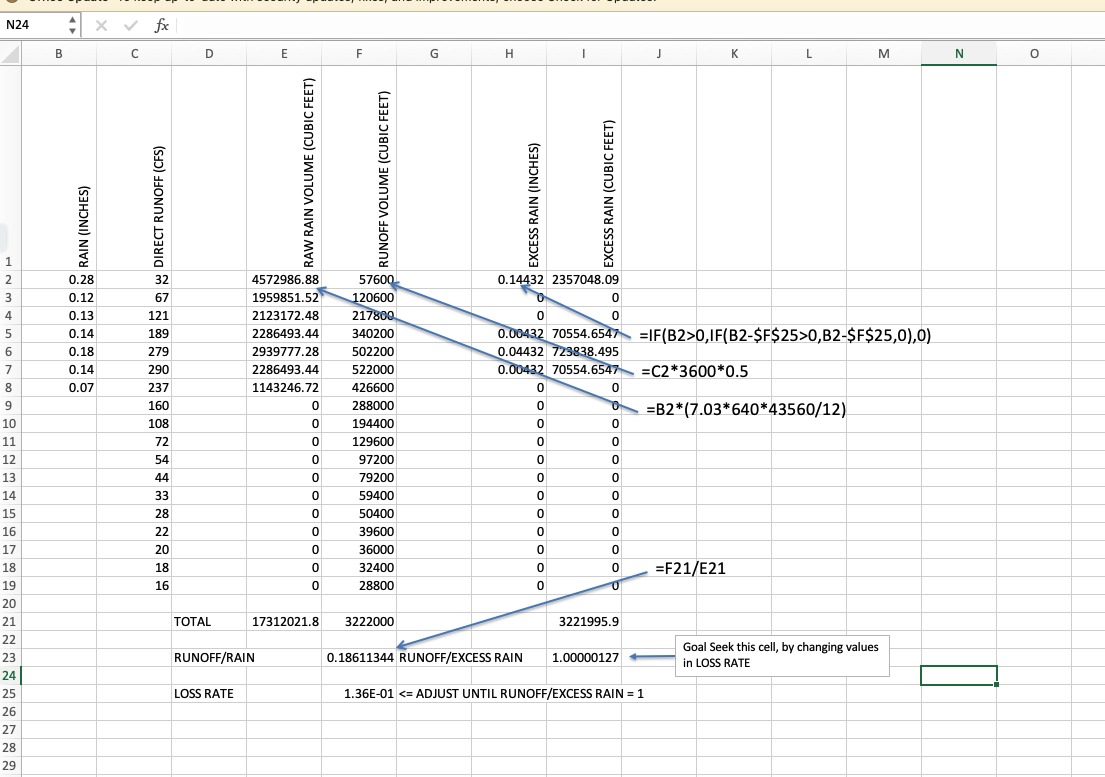
\includegraphics[width=6in]{VolumeBalance.png} 
   \caption{Volume Balance for Shoal Creek data to infer constant loss rate}
   \label{fig:VolumeBalance}
\end{figure}

\clearpage
%%%%%%%%%%%%%%%%%%%%%%%%%%%%%%%%%%%

\item Use the Matrix-Vector representation and ordinary-least-squares to construct a unit hydrograph for the watershed as depicted in Figure \ref{fig:UHbyRegression}.\footnote{This watershed will yield two negative ordinates; a SOLVER result is also shown.  Recall negative ordinates are not physically relevant, and require addressing.  They may simply be artifacts, or (more likely) sample aliasing.}

\begin{figure}[h!] %  figure placement: here, top, bottom, or page
   \centering
   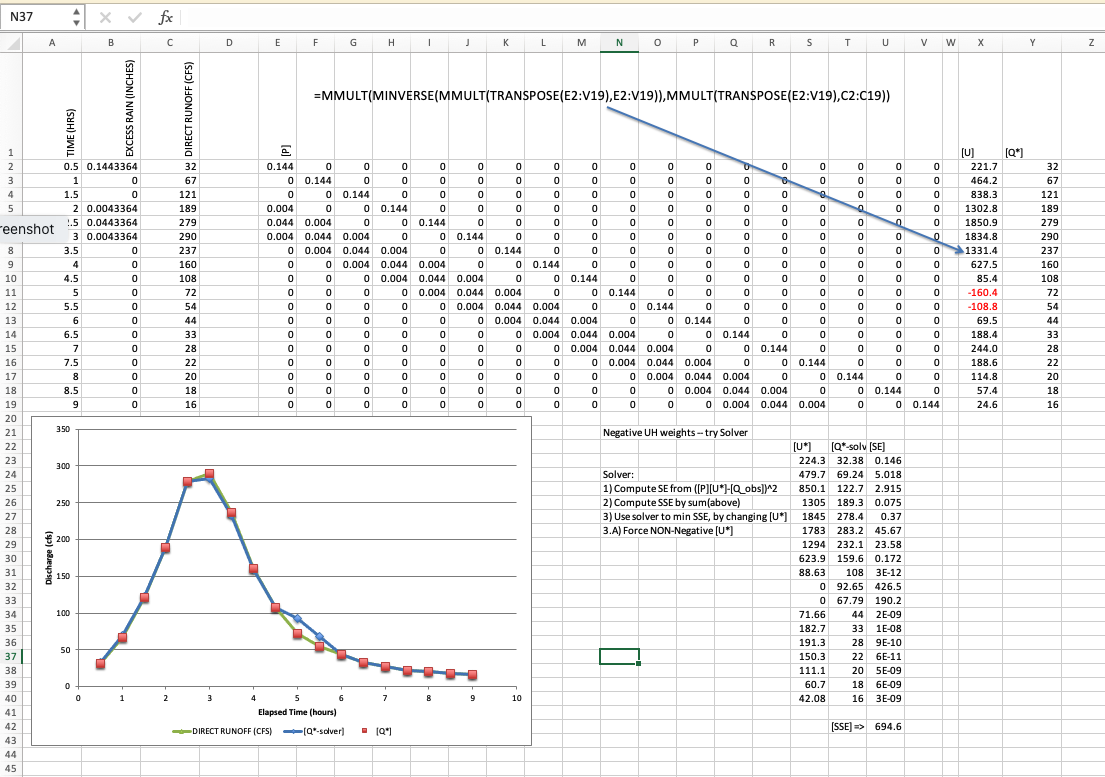
\includegraphics[width=6in]{UHbyRegression.png} 
   \caption{Spreadsheet solution}
   \label{fig:UHbyRegression}
\end{figure}

The working spreadsheet is located at \url{http://54.243.252.9/ce-3354-webroot/2-Exercises/ES-6/ES6-SourceCode/ES6-Solution.xlsx}. Figure \ref{fig:UHfromDrawings} is captured from Tab Sheet ``P2-UH-CL-LOSS-FIT''

\end{enumerate}
\end{enumerate}

\end{document}  